\documentclass[fleqn, a4paper, 12pt, twoside]{article}

\newcounter{recitationcount} %creates a new counter for recitation numbers (must be executed before exsheets is loaded)
\newcommand\recitation{\refstepcounter{recitationcount}}

\usepackage[counter-within = recitationcount]{exsheets}
\usepackage{amsmath, amssymb, amsthm} %standard AMS packages
\usepackage{marginnote} %marginnotes
\usepackage{gensymb} %miscellaneous symbols
\usepackage{commath} %differential symbols
\usepackage{xcolor} %colours
\usepackage{cancel} %cancelling terms
\usepackage{siunitx} %formatting units
\usepackage{tikz, pgfplots} %diagrams
	\usetikzlibrary{calc, hobby, patterns, intersections}
\usepackage{graphicx} %inserting graphics
\usepackage{hyperref} %hyperlinks
\usepackage{datetime} %date and time
\usepackage{ulem} %underline for \emph{}
\usepackage{xfrac, lmodern} %inline fractions
\usepackage{enumerate} %numbered lists
\usepackage{float} %inserting floats
\usepackage{circuitikz} %circuit diagrams

\newcommand\numberthis{\addtocounter{equation}{1}\tag{\theequation}} %adds numbers to specific equations in non-numbered list of equations

\newcommand{\AxisRotator}[1][rotate=0]{
	\tikz [x=0.25cm,y=0.60cm,line width=.2ex,-stealth,#1] \draw (0,0) arc (-150:150:1 and 1);%
} %rotation symbols on axes

\theoremstyle{definition}
\newtheorem{example}{Example}
\newtheorem{definition}{Definition}

\theoremstyle{theorem}
\newtheorem{theorem}{Theorem}

\newcommand{\curl}{\mathrm{curl\,}}

\makeatletter
\@addtoreset{section}{part} %resets section numbers in new part
\makeatother

\makeatletter
\newcommand*{\relrelbarsep}{.386ex}
\newcommand*{\relrelbar}{%
  \mathrel{%
    \mathpalette\@relrelbar\relrelbarsep
  }%
}
\newcommand*{\@relrelbar}[2]{%
  \raise#2\hbox to 0pt{$\m@th#1\relbar$\hss}%
  \lower#2\hbox{$\m@th#1\relbar$}%
}
\providecommand*{\rightrightarrowsfill@}{%
  \arrowfill@\relrelbar\relrelbar\rightrightarrows
}
\providecommand*{\leftleftarrowsfill@}{%
  \arrowfill@\leftleftarrows\relrelbar\relrelbar
}
\providecommand*{\xrightrightarrows}[2][]{%
  \ext@arrow 0359\rightrightarrowsfill@{#1}{#2}%
}
\providecommand*{\xleftleftarrows}[2][]{%
  \ext@arrow 3095\leftleftarrowsfill@{#1}{#2}%
}
\makeatother

\newcommand\blfootnote[1]{%
	\begingroup
	\renewcommand\thefootnote{}\footnote{#1}%
	\addtocounter{footnote}{-1}%
	\endgroup
}

\RenewQuSolPair{question}[name=Recitation \therecitationcount\ -- Exercise]{solution}[name=Recitation \therecitationcount\ -- Solution]

\SetupExSheets{solution/print = true, totoc = true} %prints all solutions by default

%opening
\title{Differential and Integral Calculus : Recitations}
\author{Aakash Jog}
\date{2014-15}

\begin{document}

\maketitle
%\setlength{\mathindent}{0pt}

\blfootnote
{	
	\begin{figure}[H]
		
\includegraphics[height = 12pt]{cc.eps}
		\includegraphics[height = 12pt]{by.eps}
		\includegraphics[height = 12pt]{nc.eps}
		
\includegraphics[height = 12pt]{sa.eps}
	\end{figure}
	This work is licensed under the Creative Commons Attribution-NonCommercial-ShareAlike 4.0 International License. To view a copy of this license, visit \url{http://creativecommons.org/licenses/by-nc-sa/4.0/}.
} %CC-BY-NC-SA license

\tableofcontents

\newpage
\section{Instructor Information}

\textbf{Michael Bromberg}\\
~\\
E-mail: \href{mailto:micbromberg@gmail.com}{micbromberg@gmail.com}\\

\newpage

\part{Sequences and Series}

\section{Sequences}

\recitation

\begin{question}
	Prove:
	\begin{equation*}
		\lim\limits_{n \to \infty} \dfrac{2n^2 + n + 1}{n^2 + 3} = 2
	\end{equation*}
\end{question}

\begin{solution}[print]
	Let
	\begin{equation*}
		\varepsilon > 0
	\end{equation*}

	\begin{align*}
		\left| \dfrac{2n^2 + n + 1}{n^2 + 3} - 2 \right| &= \left| \dfrac{2n^2 + n + 1 - 2n^2 - 6}{n^2 + 3} \right|\\
		&= \left| \dfrac{n - 5}{n^2 + 3} \right| \\
		&\leq \left| \dfrac{n - 5}{n^2} \right|\\
		&\leq \dfrac{1}{n}\\
		&< \varepsilon
	\end{align*}
	Therefore, let $N = \left[ \dfrac{1}{\varepsilon} \right] + 1$.
	Hence, for this $N$, $|a_n - L| < \varepsilon$.\\
	Therefore, $\lim\limits_{n \to \infty} \dfrac{2n^2 + n + 1}{n^2 + 3} = 2$.
	\qed
\end{solution}

\begin{question}
	Prove
	\begin{equation*}
		\lim\limits_{n \to \infty} \dfrac{n^3 + \sin n + n}{2n^4} = 0
	\end{equation*}
\end{question}

\begin{solution}[print]
	Let $\varepsilon > 0$
	\begin{align*}
		\left| \dfrac{n^3 + \sin n + n}{2n^4} \right| &\leq \left| \dfrac{n^3 + 1 + n}{2n ^4} \right|\\
		&\leq \left| \dfrac{3n^3}{2n^4} \right| = \dfrac{3}{2} \cdot \dfrac{1}{n} < \varepsilon
	\end{align*}
	Therefore, let $N = \left[ \dfrac{3}{2 \varepsilon} \right] + 1$.
	Hence, for this $N$, $|a_n - L| < \varepsilon$.\\
	Therefore, $\lim\limits_{n \to \infty} \dfrac{n^3 + \sin n + n}{2n^4} = 0$
	\qed
\end{solution}

\begin{question}
	Calculate $\sqrt[3]{n^3 + 3n} - n$.
\end{question}

\begin{solution}[print]
	\begin{align*}
		a^n - b^n = (a - b) \cdot (a^{n - 1} + a^{n - 2} b + \dots + a b^{n - 2} + b^{n - 1})
	\end{align*}
	Therefore, let
	\begin{align*}
		a &= \sqrt[3]{n^3 + 3n}\\
		b &= \sqrt[3]{n^3}
	\end{align*}

	\begin{align*}
		a - b &= \dfrac{a^3 - b^3}{a^2 + a b + b^2}\\
		\therefore \sqrt[3]{n^3 + 3n} - n &= \dfrac{n^3 + 3n - n^3}{(n^3 + 3n)^{\sfrac{2}{3}} + (n^3 + 3n)^{\sfrac{1}{3}} n + n^2}\\
		&= \dfrac{3}{\left( \dfrac{n^3 + 3n}{n^{\sfrac{3}{2}}} \right)^{\sfrac{2}{3}} + \left( \dfrac{n^3 + 3n}{n^3} \right)^{\sfrac{1}{3} n} + n}
	\end{align*}
	Therefore, the limit is 0.
\end{solution}

\begin{question}
	Prove
	\begin{equation*}
		\lim\limits_{n \to \infty} \dfrac{n!}{n^n} = 0
	\end{equation*}
\end{question}

\begin{solution}[print]
	\begin{equation*}
		0 \leq \dfrac{n!}{n^n} = \dfrac{1}{n} \dfrac{2}{n} \dots \dfrac{n}{n} \leq \dfrac{1}{n}\\
	\end{equation*}
	Therefore, by the Sandwich Theorem, $\lim\limits_{n \to \infty} \dfrac{n!}{n^n} = 0$.
\end{solution}

\begin{question}
	Let $a_1 = 3$, $a_{n + 1} = 1 + \sqrt{6 + a_n}$. Prove that $a_n$ converges and find its limit.
\end{question}

\begin{solution}[print]
	If possible, let $\lim\limits_{n \to \infty} a_n = l$.
	\begin{align*}
		a_{n + 1} &= 1 + \sqrt{6 + a_n}\\
		\intertext{Taking the limit on both sides,}
		l &= 1 + \sqrt{6 + l}\\
		\therefore l - 1 &= \sqrt{6 + l}\\
		\therefore l &= \dfrac{3 \pm \sqrt{29}}{2}
	\end{align*}
	As $a_n \geq 0$, $l = \dfrac{3 + \sqrt{29}}{2}$.
	~\\
	\begin{align*}
		a_2 &= 1 + \sqrt{6 + a_1}\\
		&= 1 + \sqrt{6 + 3}\\
		&= 4\\
		\therefore a_2 &> a_1
	\end{align*}
	If possible, let $a_n \geq a_{n - 1}$.\\
	Therefore,
	\begin{align*}
		a_{n + 1} &= 1 + \sqrt{6 + a_n}\\
		&\geq 1 + \sqrt{6 + a_{n + 1}} = a_n
	\end{align*}
	Therefore by induction, $\{a_n\}$ is monotonically increasing.
	~\\
	\begin{align*}
		a_1 &= 3\\
		\therefore a_1 \leq 5
	\end{align*}
	If possible, let $a_n \leq 5$.\\
	Therefore,
	\begin{equation*}
		a_{n + 1} = 1 + \sqrt{6 + a_n} \leq q + \sqrt{11} \leq 5
	\end{equation*}
	Therefore by induction, $\{a_n\}$ is bounded from above by 5.
\end{solution}

\recitation

\subsection{Limit of a Function by Heine}

\begin{definition}
	\begin{equation*}
		\lim\limits_{x \to x_0} f(x) = l
	\end{equation*}
	if for every sequence $x_n$, such that $\lim\limits_{n \to \infty} x_n = x_0$, \begin{equation*}
		\lim\limits_{n \to \infty} f(x_n) = l
	\end{equation*}
\end{definition}

\begin{theorem}
	If $f$ is continuous at $x_0$ and $x_n \to x_0$, then 
	\begin{equation*}
		\lim\limits_{n \to \infty} f(x_n) = f\left( \lim\limits_{n \to \infty} x_n \right) = f_{x_0}
	\end{equation*}
\end{theorem}

\begin{question}
	Calculate $\lim\limits_{n \to \infty} \sqrt[n]{n}$.
\end{question}

\begin{solution}
	Let
	\begin{equation*}
		f(x) = x^{\sfrac{1}{x}}
	\end{equation*}
	Therefore,
	\begin{align*}
		\lim\limits_{x \to \infty} x^{\sfrac{1}{x}} &= \lim\limits_{x \to \infty} e^{\cancelto{0}{\dfrac{\ln x}{x}}}\\
		&= 1
	\end{align*}
\end{solution}

\subsection{Sub-sequences}

\begin{question}
	Find all partial limits and $\overline{\lim}$ and $\underline{\lim}$ of
	\begin{equation*}
		a_n = \left( \cos \dfrac{\pi n}{4} \right)^n
	\end{equation*}
\end{question}

\begin{solution}
	Let $k, z \in \mathbb{Z}$
	\begin{align*}
		\cos \dfrac{\pi n}{4} &= \cos \dfrac{\pi (n + k)}{4}\\
		\therefore \dfrac{\pi n}{4} &= \dfrac{\pi (n + k)}{4} + 2 \pi z\\
		\therefore \pi n &= \pi (n + k) + 8 \pi z\\
		\therefore k &= 8 z
	\end{align*}
	Therefore,
	\begin{align*}
		a_{8k} &= \left( \cos \dfrac{\pi \cdot 8k}{4} \right)^{8k}\\
		&= \left( \cos (2 \pi k) \right)^{8k}\\
		&= 1\\
		a_{8k + 1} &= \left( \cos \dfrac{\pi \cdot (8k + 1)}{4} \right)^{8k + 1}\\
		&= \left( \cos \dfrac{\pi}{4} \right)^{8k + 1}\\
		&= \left( \dfrac{\sqrt{2}}{2} \right)^{8k + 1}\\
		a_{8k + 2} &= \left( \cos \dfrac{\pi \cdot (8k + 2)}{4} \right)^{8k + 2}\\
		&= \left( \cos \dfrac{\pi}{2} \right)^{8k + 2}
	\end{align*}
	Therefore,
	\begin{align*}
		\lim\limits_{k \to \infty} a_{8k} &= 1\\
		\lim\limits_{k \to \infty} a_{8k + 1} &= \lim\limits_{k \to \infty} \left( \dfrac{\sqrt{2}}{2} \right)^{8k + 1}\\
		&= 0
	\end{align*}
	Similarly,
	\begin{align*}
		\lim\limits_{k \to \infty} a_{8k + 2} &= 0\\
		\lim\limits_{k \to \infty} a_{8k + 3} &= 0\\
		\lim\limits_{k \to \infty} a_{8k + 4} &= \lim\limits_{k \to \infty} (-1)^{8k + 4}\\
		&= 1\\
		\lim\limits_{k \to \infty} a_{8k + 5} &= 0\\
		\lim\limits_{k \to \infty} a_{8k + 6} &= 0\\
		\lim\limits_{k \to \infty} a_{8k + 7} &= 0
	\end{align*}
	Therefore, $\{a_n\}$ has two partial limits, $0$ and $1$.
	\begin{align*}
		\overline{\lim} a_n &= 1\\
		\underline{\lim} a_n &= 0
	\end{align*}
\end{solution}

\section{Series}

\begin{definition}[Convergence of a series]
	Let $\{a_n\}$ be a sequence. Let $S_n$ be a sequence of partial sums of $a_n$, s.t.
	\begin{equation*}
		S_n = \sum_{k = 1}^{n} a_k
	\end{equation*}
	The series $\sum_{k = 1}^{\infty} a_k$ is said to converge to $l$ if
	\begin{equation*}
		\lim\limits_{n \to \infty} S_n = l
	\end{equation*}
	that is,
	\begin{equation*}
		\sum_{k = 1}^{\infty} a_k = \lim\limits_{n \to \infty} \sum_{k = 1}^{n} a_k = \lim\limits_{n \to \infty} S_n
	\end{equation*}
\end{definition}

\begin{question}
	Does $\displaystyle \sum_{k = 0}^{\infty} q^k$ where $-1 < q < 1$ converge?
\end{question}

\begin{solution}
	\begin{align*}
		\sum_{k = 0}^{\infty} q^k &= \lim\limits_{n \to \infty} \sum_{k = 0}^{n} q^k\\
		&= \lim\limits_{n \to \infty} \dfrac{1 - q^{n + 1}}{1 - q}\\
		&= \dfrac{1}{1 - q}
	\end{align*}
	Therefore, the series converges.
\end{solution}

\begin{question}
	Does $\displaystyle \sum_{k = 1}^{\infty} \dfrac{1}{k(k + 1)}$ converge?
\end{question}

\begin{solution}
	\begin{align*}
		\sum_{k = 1}^{\infty} \dfrac{1}{k(k + 1)} &= \sum_{k = 1}^{\infty} \left( \dfrac{1}{k} - \dfrac{1}{k + 1} \right)\\
		&= \lim\limits_{n \to \infty} \sum_{k = 1}^{n} \left( \dfrac{1}{k} - \dfrac{1}{k + 1} \right)\\
		&= \lim\limits_{n \to \infty} \left( 1 - \dfrac{1}{n + 1} \right)\\
		&= 1
	\end{align*}
\end{solution}

\begin{question}
	Does $\displaystyle \sum_{k = 1}^{\infty} \left( 1 + \dfrac{1}{k} \right)^k$ converge?
\end{question}

\begin{solution}
	\begin{align*}
		\lim\limits_{k \to \infty} \left( 1 + \dfrac{1}{k} \right)^k &= e\\
		\therefore \lim\limits_{k \to \infty} \left( 1 + \dfrac{1}{k} \right)^k &\neq 0
	\end{align*}
	Therefore, the necessary condition is nt satisfied.
	Hence, the series does not converge.
\end{solution}

\subsection{Comparison Tests for Positive Series}

\begin{theorem}[First Comparison Test]
	If $a_n \ge 0$, $b_n \ge 0$, and $a_n \le b_n$, then
	\begin{enumerate}
		\item If $\sum b_n$ converges, then $\sum a_n$ converges.
		\item If $\sum a_n$ diverges, then $\sum b_n$ diverges.
	\end{enumerate}
	\label{First_Comparison_Test}
\end{theorem}

\begin{theorem}[Second Comparison Test]
	If $a_n \ge 0$, $b_n \ge 0$ and
	\begin{equation*}
		\lim\limits_{n \to \infty} \dfrac{a_n}{b_n} = l
	\end{equation*}
	where $0 < l < \infty$, then $\sum a_n$ and $\sum b_n$ converge or diverge simultaneously.
	\label{Second_Comparison_Test}
\end{theorem}

\recitation

\begin{question}
	Suppose the sequence $a_n$ satisfies the condition
	\begin{equation*}
		a_{n + 1} - a_n > \dfrac{1}{n}
	\end{equation*}
	$\forall n \in \mathbb{N}$.\\
	Prove that $\lim\limits_{n \to \infty} a_n = \infty$.
\end{question}

\begin{solution}
	\begin{align*}
		a_{n + 1} &= a_{n + 1} - a_{n} + a_{n} - a_{n - 1} + a_{n - 1} - a_{n - 2} + \dots + a_{2} - a_{1} + a_{1}\\
		&= \sum_{k = 1}^{n} \left( a_{k + 1} - a_{k} \right) + a_{1}\\
		&\ge \sum_{k = 1}^{n} \dfrac{1}{k} + a_1
	\end{align*}
	As the harmonic series diverges, $\sum\limits_{k = 1}^{n} \dfrac{1}{k} + a_1$ diverges.\\
	Therefore, by the \nameref{First_Comparison_Test}, $\sum\limits_{k = 1}^{\infty} (a_{k + 1} - a_k)$ diverges.
\end{solution}

\begin{question}
	Check the convergence of $\sum\limits_{n = 2}^{\infty} \dfrac{n + \sin n}{n^3 + \cos \pi n}$.
\end{question}

\begin{solution}
	The series is non-negative.
	Therefore, the comparison tests are applicable.
	\begin{align*}
		\dfrac{n + \sin n}{n^3 + \cos \pi n} &\le \dfrac{n + 1}{n^3 - 1}\\
		\therefore \dfrac{n + \sin n}{n^3 + \cos \pi n} &\le \dfrac{2n}{n^3 - \dfrac{n^3}{2}} &\le \dfrac{4}{n^2}
	\end{align*}
	Therefore, by the \nameref{First_Comparison_Test}, as $\dfrac{4}{n^2}$ converges, $\sum_{n = 2}^{\infty} \dfrac{n + \sin n}{n^3 + \cos \pi n}$ also converges.
\end{solution}

\begin{question}
	Let $a_n \ge 0$ and suppose that $\sum a_n$ converges. Prove that $\sum {a_n}^2$ converges.\\
	Is it true without the assumption $a_n \ge 0$?
\end{question}

\begin{solution}
	As $\sum a_n$ converges, $\lim\limits_{n \to \infty} a_n = 0$.\\
	Therefore, $\exists N \in \mathbb{N}$, such that $\forall n > N$, $a_n < 1$.\\
	Therefore, $\forall n > N$, ${a_n}^2 \le a_n$.
	Hence, as $\sum\limits_{n = N + 1}^{\infty} a_n$ converges, $\sum\limits_{n = N + 1}^{\infty} {a_n}^2$ also converges.
	Hence, $\sum\limits_{n = 1}^{\infty} a_n$ also converges.\\
	~\\
	This is not true without the assumption $a_n \ge 0$, as the argument ${a_n}^2 \le a_n$ does not hold.
\end{solution}

\begin{question}
	For which $\alpha$ does $\sum \left( \sqrt{n + 1} - \sqrt{n} \right)^{\sfrac{\alpha}{2}}$ converge?
\end{question}

\begin{solution}
	\begin{align*}
		\sum \left( \sqrt{n + 1} - \sqrt{n} \right)^{\sfrac{\alpha}{2}} &= \sum \left( \dfrac{n + 1 - n}{\sqrt{n + 1} + \sqrt{n}} \right)^{\sfrac{\alpha}{2}}\\
		&= \sum \left( \dfrac{1}{\sqrt{n + 1} - \sqrt{n}} \right)^{\sfrac{\alpha}{2}}
	\end{align*}
	The series is positive.
	Therefore, the comparison tests are applicable.\\
	Comparing with $\left( \dfrac{1}{\sqrt{n}} \right)^{\sfrac{\alpha}{2}}$,
	\begin{align*}
		\dfrac{\left( \dfrac{1}{\sqrt{n + 1} + \sqrt{n}} \right)^{\sfrac{\alpha}{2}}}{\left( \dfrac{1}{\sqrt{n}} \right)^{\sfrac{\alpha}{2}}} &= \left( \dfrac{\sqrt{n}}{\sqrt{n + 1} + \sqrt{n}} \right)^{\sfrac{\alpha}{2}}\\
		\therefore \lim\limits_{n \to \infty} \left( \dfrac{\sqrt{n}}{\sqrt{n + 1} + \sqrt{n}} \right)^{\sfrac{\alpha}{2}} &= \left( \dfrac{1}{2} \right)^{\sfrac{\alpha}{2}}
	\end{align*}
	$\sum \dfrac{1}{n^{\sfrac{\alpha}{2}}}$ converges if and only if $\dfrac{\alpha}{4} > 1$, i.e. if an inly if $\alpha > 4$.\\
	By the \nameref{Second_Comparison_Test}, $\sum \dfrac{1}{n^{\sfrac{\alpha}{4}}}$ and the series converge or diverge simultaneously.\\
	Therefore, the series converges for $\alpha > 4$.
\end{solution}

\begin{question}
	Check the convergence of $\sum\limits_{n = 1}^{\infty} \sin \dfrac{1}{n}$.
\end{question}

\begin{solution}
	$\forall n \in \mathbb{N}$, $\sin \dfrac{1}{n} \ge 0$\\
	\begin{align*}
		\lim\limits_{n \to \infty} \dfrac{\sin \dfrac{1}{n}}{\dfrac{1}{n}} &= 1
	\end{align*}
	Therefore, by \nameref{Second_Comparison_Test}, $\sum \dfrac{1}{n}$ and $\sum \sin \dfrac{1}{n}$ diverge simultaneously.
\end{solution}

\subsection{d'Alembert Criteria (Ratio Test)}

\begin{definition}[Absolute and conditional convergence]
	The series $\sum a_n$ is said to converge absolutely if $\sum |a_n|$ converges.
	The series $\sum a_n$ is said to converge conditionally if it converges but $\sum |a_n|$ diverges.
\end{definition}

\begin{theorem}
	If the series $\sum a_n$ converges absolutely then it converges.
\end{theorem}

\begin{theorem}[d'Alembert Criteria (Ratio Test)]
	\begin{enumerate}
		\item 
			If 
			\begin{equation*}
			\lim\limits_{n \to \infty} \left| \dfrac{a_{n - 1}}{a_n} \right| = L < 1
			\end{equation*}
			then $\sum a_n$ converges absolutely.
		\item 
			If 
			\begin{equation*}
			\lim\limits_{n \to \infty} \left| \dfrac{a_{n - 1}}{a_n} \right| = L > 1
			\end{equation*}
			(including $L = \infty$), then $\sum a_n$ converges diverges.
		\item If $L = 1$, the test does not apply.
	\end{enumerate}
	\label{d'Alembert_Criteria_(Ratio_Test)}
\end{theorem}

\begin{question}
	Check the convergence of $\sum \dfrac{(-1)^n \cdot n^{1000}}{1 \cdot 3 \cdot 5 \cdot \dots \cdot (2n - 1)}$.
\end{question}

\begin{solution}
	\begin{align*}
	\sum_{n = 1}^{\infty} \left| \dfrac{(-1)^n \cdot n^{1000}}{1 \cdot \dots \cdot (2n - 1)} \right| &= \sum_{n = 1}^{\infty} \dfrac{n^{1000}}{1 \cdot \dots \cdot (2n - 1)}
	\end{align*}
	Therefore, by the \nameref{d'Alembert_Criteria_(Ratio_Test)},
	\begin{align*}
		\dfrac{a_{n + 1}}{a_n} &= \dfrac{\dfrac{(n + 1)^{1000}}{1 \cdot \dots \cdot (2n + 1)}}{\dfrac{n^{1000}}{1 \cdot \dots \cdot (2n - 1)}}\\
		&= \left( \dfrac{n + 1}{n} \right)^{1000} \cdot \dfrac{1}{2n + 1}\\
		\therefore \lim\limits_{n to \infty} \left( \dfrac{n + 1}{n} \right)^{1000} \cdot \dfrac{1}{2n + 1} &= 0\\
		\therefore \left( \dfrac{n + 1}{n} \right)^{1000} \cdot \dfrac{1}{2n + 1} &< 1
	\end{align*}
	Therefore, by the \nameref{d'Alembert_Criteria_(Ratio_Test)}, the series converges absolutely, and hence converges.
\end{solution}

\subsection{Cauchy Criteria (Cauchy Root Test)}

\begin{theorem}[Cauchy Criteria (Cauchy Root Test)]
	\begin{enumerate}
		\item
			If 
			\begin{equation*}
			\overline{\lim} \sqrt[n]{|a_n|} = L < 1
			\end{equation*}
			then $\sum a_n$ converges absolutely.
		\item
			If 
			\begin{equation*}
			\overline{\lim} \sqrt[n]{|a_n|} = L > 1
			\end{equation*}
			(including $L = \infty$), then $\sum a_n$ diverges.
		\item If $L = 1$, the test does not apply.
	\end{enumerate}
	\label{Cauchy_Criteria_(Cauchy_Root_Test)}
\end{theorem}

\begin{question}
	Check the convergence of $\sum \left( 1 - \dfrac{2}{n} \right)^{n^2}$.
\end{question}

\begin{solution}
	\begin{align*}
		\sqrt[n]{\left( 1 - \dfrac{2}{n} \right)^{n^2}} &= \left( 1 - \dfrac{2}{n} \right)^n\\
		\therefore \lim\limits_{n \to \infty} \left( 1 - \dfrac{2}{n} \right)^n &= e^{-2}\\
		\therefore \lim\limits_{n \to \infty} \left( 1 - \dfrac{2}{n} \right)^n &< 1
	\end{align*}
	Therefore, by the \nameref{Cauchy_Criteria_(Cauchy_Root_Test)}, $\sum \left( 1 - \dfrac{2}{n} \right)^{n^2}$ converges.
\end{solution}

\subsection{Leibniz's Criteria}

\begin{definition}[Alternating series]
	The series $\sum\limits_{n = 1}^{\infty} (-1)^{n - 1} a_n$, where all $a_n > 0$ or all $a_n < 0$ is called an alternating series.
\end{definition}

\begin{theorem}[Leibniz's Criteria for Convergence]
	If an alternating series $\sum (-1)^{n - 1} a_n$ with $a_n > 0$ satisfies
	\begin{enumerate}
		\item $a_{n + 1} \le a_n$, i.e. $\{a_n\}$ is monotonically decreasing.
		\item $\lim\limits_{n \to \infty} a_n = 0$
	\end{enumerate}
	then the series $(-1)^{n - 1} a_n$ converges.
	\label{Leibniz's_Criteria_for_Convergence}
\end{theorem}

\begin{question}
	Prove or disprove: There exists $\{a_n\}$, such that $\sum a_n$ converges and $\sum (1 + a_n) a_n$ diverges.
\end{question}

\begin{solution}
	Let $a_n = \dfrac{(-1)^n}{\sqrt{n}}$.\\
	Therefore, by \nameref{Leibniz's_Criteria_for_Convergence}, $\sum \dfrac{(-1)^n}{\sqrt{n}}$ converges.\\
	\begin{align*}
		\sum (1 + a_n) a_n &= \sum \left( 1 + \dfrac{(-1)^n}{\sqrt{n}} \right) \dfrac{(-1)^n}{\sqrt{n}}\\
		&= \sum \left( \dfrac{(-1)^n}{\sqrt{n}} + \dfrac{1}{n} \right)
	\end{align*}
	Therefore, as $\sum \dfrac{1}{n}$ diverges, and $\sum \dfrac{(-1)^n}{\sqrt{n}}$ converges, $\sum \left( \dfrac{1}{n} + \dfrac{(-1)^n}{\sqrt{n}} \right)$ diverges.
\end{solution}

\subsection{Integral Test}

\begin{theorem}[Integral Test]
	If $f(x) : [1, \infty) \to [0, \infty)$ is monotonically decreasing.
	Then, $\sum\limits_{n = 1}^{\infty} f(n)$ and $\int\limits_{1}^{\infty} f(x) \dif x$ converge or diverge simultaneously.
	\label{Integral_Test}
\end{theorem}

\begin{question}
	Check the convergence of $\sum\limits_{n = 2}^{\infty} \dfrac{1}{n \ln n}$
\end{question}

\begin{solution}
	Let
	\begin{align*}
		f(x) &= \dfrac{1}{x \ln x}
	\end{align*}
	$f(x)$ is monotonically decreasing.
	Therefore, the \nameref{Integral_Test} is applicable.\\
	Therefore,
	\begin{align*}
		\int\limits_{2}^{\infty} \dfrac{1}{x \ln x} \dif x &= \int\limits_{\ln 2}^{\infty} \dfrac{1}{y} \dif y\\
		&= \left. \ln y \right|_{\ln 2}^{\infty}\\
		&= \infty
	\end{align*}
	Therefore, by the integral test, $\sum \dfrac{1}{n \ln n}$ diverges.
\end{solution}

\recitation

\subsection*{}

\begin{question}
	Let $d_n \ge 0$ and suppose 
	\begin{equation*}
		\sum\limits_{n = 0}^{\infty} d_n = \infty
	\end{equation*}
	Prove that
	\begin{equation*}
		\sum_{n = 0}^{\infty} \dfrac{d_n}{1 + d_n} = \infty
	\end{equation*}
\end{question}

\begin{solution}
	If possible, let $d_n$ be a bounded sequence.
	Then there exists $M$, such that $d_n \le M$, $\forall n \in \mathbb{N}$.\\
	Therefore,
	\begin{align*}
		\dfrac{d_n}{1 + d_n} &\ge \dfrac{d_n}{1 + M}
	\end{align*}
	Therefore, by the \nameref{Second_Comparison_Test}, as $\sum d_n$ diverges, $\sum \dfrac{d_n}{1 + d_n}$ also diverges.\\
	~\\
	If $d_n$ is not bounded, then there is a subsequence $d_{n_k}$ which diverges.
	Therefore,
	\begin{align*}
		\dfrac{d_{n_k}}{1 + d_{n_k}} &= \dfrac{1}{\dfrac{1}{d_{n_k}} + 1}\\
		\therefore \lim\limits_{k \to \infty} \dfrac{d_{n_k}}{1 + d_{n_k}} &= 1
	\end{align*}
	Therefore,
	\begin{align*}
		\lim\limits_{n \to \infty} \dfrac{d_n}{1 + d_n} &\neq 0
	\end{align*}
	Therefore, the necessary condition for convergence is not fulfilled.
	Therefore, the series converges.
\end{solution}

\begin{question}
	Let
	\begin{equation*}
		d_n = 
			\begin{cases}
				1 &;\quad n = k^2, k \in \mathbb{N}\\
				0 &;\quad n \neq k^2, k \in \mathbb{N}\\
			\end{cases}
	\end{equation*}
	Does $\sum \dfrac{d_n}{1 + n \cdot d_n}$ diverge?
\end{question}

\begin{solution}
	\begin{align*}
		d_n &= 
			\begin{cases}
				1 &;\quad n = k^2, k \in \mathbb{N}\\
				0 &;\quad n \neq k^2, k \in \mathbb{N}\\
			\end{cases}\\
		\therefore \dfrac{d_n}{1 + n \cdot d_n} &=
			\begin{cases}
				\dfrac{1}{1 + k^2} &;\quad n = k^2, k \in \mathbb{N}\\
				0 &;\quad n \neq k^2, k \in \mathbb{N}\\
			\end{cases}
	\end{align*}
	As $\dfrac{1}{1 + k^2} \le \dfrac{1}{k^2}$ and as $\dfrac{1}{k^2}$ converges, $\sum \dfrac{1}{1 + k^2}$ also converges.
\end{solution}

\begin{question}
	Let $a_n$ be a sequence such that $|a_{n + 1} - a_n| \le b_{n + 1}$ for all $n \in \mathbb{N}$ where $\sum b_k$ converges.
	Prove that $\{a_n\}$ converges.
\end{question}

\begin{solution}
	Let $\varepsilon > 0$.
	\begin{align*}
		|a_m - a_n| &= |a_m - a_{m - 1} + a_{m - 1} + \dots - a_n|\\
		&\le \sum_{k = n + 1}^{m} |a_k - a_{k - 1}|\\
		&\le \sum_{k = n + 1}^{m} b_k
	\end{align*}
	Therefore, as $\sum b_n$ converges, the series satisfies the \nameref{Cauchy_Criteria_(Cauchy_Root_Test)}.
	Therefore, there exists $N$, such that $\forall m > n > N, \left| \sum\limits_{k = n + 1}^{m} b_k \right| < \varepsilon$.
	Therefore, for $m > n > N$,
	\begin{equation*}
		|a_m - a_n| \le \sum_{k = n + 1}^{m} b_n < \varepsilon
	\end{equation*}
\end{solution}

\section{Power Series}

\begin{definition}[Power series]
	A power series around $x_0$ is a function of the form
	\begin{equation*}
		f(x) = \sum_{n = 0}^{\infty} a_n (x - x_0)^n
	\end{equation*}
	where $\{a_n\}$ is a sequence of real numbers.
\end{definition}

\begin{theorem}[Abel's Theorem]
	For every power series $\sum a_n (x - x_0)^n$, there exists $R \in [0,\infty]$, such that for all $x$ satisfying $|x - x_0| < R$, the series converges and for all $x$ satisfying $|x - x_0| > R$ the series diverges.
	\label{Abel's_Theorem}
\end{theorem}

\begin{theorem}[Cauchy's Formula for Radius of Convergence]
	\begin{equation*}
		R = \dfrac{1}{\overline{\lim} \sqrt[n]{|a_n|}}
	\end{equation*}
	\label{Cauchy's_Formula_for_Radius_of_Convergence}
\end{theorem}

\begin{theorem}[Hadamard's Formula for Radius of Convergence]
	If $\lim\limits_{n \to \infty} \left| \dfrac{a_n}{a_{n + 1}} \right|$ exists, then
	\begin{equation*}
		\lim\limits_{n \to \infty} \left| \dfrac{a_n}{a_{n + 1}} \right| = R
	\end{equation*}
	\label{Hadamard's_Formula_for_Radius_of_Convergence}
\end{theorem}

\begin{question}
	Find the domain of convergence of $\sum\limits_{n = 1}^{\infty} \dfrac{(2x - 4)^n}{n}$.
\end{question}

\begin{solution}
	\begin{align*}
		\sum_{n = 1}^{\infty} \dfrac{(2x - 4)^n}{n} &= \sum_{n = 1}^{\infty} \dfrac{2^n (x - 2)^n}{n}
	\end{align*}
	Therefore, by \nameref{Cauchy's_Formula_for_Radius_of_Convergence},
	\begin{align*}
		R &= \dfrac{1}{\overline{\lim} \sqrt[n]{|a_n|}}\\
		&= \dfrac{1}{\lim\limits_{n \to \infty} \sqrt[n]{\dfrac{2^n}{n}}}\\
		&= \dfrac{1}{\lim\limits_{n \to \infty} \dfrac{2}{\sqrt[n]{n}}}\\
		&= \dfrac{1}{2}
	\end{align*}
	Therefore, the series converges for
	\begin{equation*}
		|x - 2| < \dfrac{1}{2}
	\end{equation*}
	and diverges for
	\begin{equation*}
		|x - 2| > \dfrac{1}{2}
	\end{equation*}
	If $x = \dfrac{5}{2}$, 
	\begin{align*}
		\sum_{n = 1}^{\infty} \dfrac{2^n}{n} \left( \dfrac{5}{2} - 2 \right)^n\\
		&= \sum_{n = 1}^{\infty} \dfrac{1}{n}
	\end{align*}
	Therefore, the series diverges.\\
	If $x = \dfrac{3}{2}$, 
	\begin{align*}
		\sum_{n = 1}^{\infty} \dfrac{2^n}{n} \left( \dfrac{3}{2} - 2 \right)^n\\
		&= \sum_{n = 1}^{\infty} (-1)^n \dfrac{1}{n}
	\end{align*}
	Therefore, by \nameref{Leibniz's_Criteria_for_Convergence}, the series converges.\\
	Therefore, the domain of convergence is $\left[ \dfrac{3}{2} , \dfrac{5}{2} \right)$.
\end{solution}

\begin{question}
	Find the radius of convergence of $\sum\limits_{n = 0}^{\infty} n! x^{n!}$.
\end{question}

\begin{solution}
	\begin{align*}
		\dfrac{1}{\overline{\sqrt[n]{a_n}}} &= x + x + 2 x^2 + 6 x^6 + 24 x^{24} + \dots
	\end{align*}
	Therefore,
	\begin{align*}
		a_n &=
			\begin{cases}
				n &;\quad n = k^2\\
				0 &;\quad n \neq k^2\\
			\end{cases}
	\end{align*}
	Therefore, 
	\begin{align*}
		R &= \dfrac{1}{\lim\limits_{n \to \infty} \sqrt[n]{a_n}}\\
		&= \dfrac{1}{\lim\limits_{k \to \infty} \sqrt[k!]{k!}}\\
		&= 1
	\end{align*}
\end{solution}

\recitation

\subsection{Power Series Representation of a Function}

\begin{theorem}
	The power series representation of a function $f(x)$ is equal to its Taylor series if and only if $\lim\limits_{n \to \infty} R_n(x) = 0$, where $R_n(x)$ is the Lagrange remainder.
\end{theorem}

\subsection{Differentiation and Integrations of Power Series}

\begin{question}
	Find the power series representation of $\tan^{-1} x$.
\end{question}

\begin{solution}
	\begin{align*}
		\dod{\tan^{-1} x}{x} &= \dfrac{1}{1 + x^2}\\
		&= \sum\limits_{n = 0}^{\infty} (-1)^n x^{2 n}\\
		\intertext{Integrating term by term,}
		\tan^{-1} x &= \sum\limits_{n = 0}^{\infty} (-1)^n \dfrac{x^{2 n + 1}}{2 n + 1} + c\\
		\intertext{As $\tan^{-1} 0 = 0$, $c = 0$. Therefore,}
		\tan^{-1} x &= \sum\limits_{n = 0}^{\infty} (-1)^n \dfrac{x^{2 n + 1}}{2 n + 1}\\
	\end{align*}
\end{solution}

\begin{question}
	Find an explicit formula for $\sum\limits_{n = 1}^{\infty} x^n n^2$.
\end{question}

\begin{solution}
	\begin{align*}
		\sum\limits_{n = 1}^{\infty} x^n n^2 &= x \cdot \sum\limits_{n = 1}^{\infty} x^{n - 1} n^2
	\end{align*}
	Let
	\begin{align*}
		g(x) &= \sum\limits_{n = 1}^{\infty} n^2 x^{n - 1}
	\end{align*}
	Integrating term by term,
	\begin{align*}
		\int g(x) \dif x &= \sum\limits_{n = 1}^{\infty} n^2 \dfrac{x^n}{n}\\
		&= \sum\limits_{n = 1}^{\infty} n x^n\\
		&= x \cdot \sum\limits_{n = 1}^{\infty} n x^{n - 1}
	\end{align*}
	Let
	\begin{align*}
		h(x) &= \sum\limits_{n = 1}^{\infty} n x^{n - 1}\\
		\therefore \int h(x) \dif x &= \dfrac{x}{1 - x}
	\end{align*}
	Therefore, inside radius of convergence $R = 1$, differentiating $\int h(x) \dif x$,
	\begin{align*}
		h(x) &= \dfrac{1 - x + x}{(1 - x)^2}\\
		&= \dfrac{1}{(1 - x)^2}\\
		\therefore \int g(x) \dif x &= x h(x)\\
		&= \dfrac{x}{(1 - x)^2}\\
		\therefore g(x) &= \dfrac{(1 - x)^2 + 2 (1 - x) x}{(1 - x)^4}\\
		\therefore \sum\limits_{n = 1}^{\infty} x^n n^2 &= x \cdot \dfrac{(1 - x)^2 + 2 (1 - x) x}{(1 - x)^4}
	\end{align*}
\end{solution}

\begin{question}
	Find the sum $\sum\limits_{n = 1}^{\infty} \dfrac{1}{n 2^n}$.
\end{question}

\begin{solution}
	Let
	\begin{align*}
		f(x) &= \sum\limits_{n = 1}^{\infty} \dfrac{x^n}{n}
	\end{align*}
	be a power series with radius $R$.\\
	Therefore,
	\begin{align*}
		\sum\limits_{n = 1}^{\infty} \dfrac{1}{n 2^n} &= f\left( \dfrac{1}{2} \right)
	\end{align*}
	Therefore,
	\begin{align*}
		f'(x) &= \sum\limits_{n = 1}^{\infty} x^{n - 1}\\
		&= \dfrac{1}{1 - x}\\
		\therefore f(x) &= -\ln (1 - x) + c\\
		\intertext{As $f(0) = 0$, $c = 0$. Therefore,}
		f(x) &= -\ln (1 - x)
	\end{align*}
	Therefore,
	\begin{align*}
		f\left( \dfrac{1}{2} \right) &= -\ln \left( \dfrac{1}{2} \right)\\
		&= \ln 2
	\end{align*}
\end{solution}

\section{Sequences of Functions}

\begin{definition}[Point-wise convergence and domain of convergence]
	$\{f_n\}$ is said to converge point-wise in some domain $E \subset D$ if $\forall x \in E$, the sequence $\{f_n(x)\}$ converges.
	In this case, $E$ is said to be a domain of convergence of $\{f_n\}$.
\end{definition}

\begin{question}
	Let $f(x) : \mathbb{R} \to \mathbb{R}$ be some function such that $\lim\limits_{x \to \infty} f(x) = 0$.
	Let $f_n(x) = f(n x)$.
	What is the domain of convergence of $f_n$?
	What is the limit function?
\end{question}

\begin{solution}
	Let $x$ be a particular number in $(0,\infty)$.
	\begin{align*} 
		\lim\limits_{n \to \infty} f_n(x) &= \lim\limits_{n \to \infty} f(n x)\\
		\intertext{Therefore, as $\lim\limits_{x \to \infty} f(x) = 0$,}
		\lim\limits_{n \to \infty} f_n(x) &= 0
	\end{align*}
	Therefore the domain of convergence is $(0,\infty)$ and the limit function is a constant $0$.\\
	~\\
	Although the all functions in $\{f_n\}$ are continuous, the limit function is not continuous.
\end{solution}

\recitation

\begin{definition}[Uniform convergence]
	A sequence of functions $\{f_n\}$ is said to converge uniformly to $f$ in the domain $E$, if $\forall \varepsilon$, $\exists N$ such that $\forall n > N$ and $\forall x \in E$, $|f_n(x) - f_(x)| < \varepsilon$.
	If $f_n$ converges to $f$ uniformly in $E$, it is denoted as $f_n \xrightrightarrows{E} f$.
\end{definition}

\subsection{Supremum and Infimum of Sets}

\begin{definition}[Supremum]
	Let $A \subseteq \mathbb{R}$ be a bounded set.
	$M$ is said to be the supremum of $A$ if
	\begin{enumerate}
		\item $\forall x \in A$, $x \le M$, i.e. $M$ is an upper bound of $A$.
		\item $\forall \varepsilon$, $\exists x \in A$, such that $x > M - \varepsilon$.
	\end{enumerate}
	That is, the supremum of $A$ is the least upper bound of $A$.\\
	The supremum may or may not be in $A$.
\end{definition}

\begin{definition}[Infimum]
	Let $A \subseteq \mathbb{R}$ be a bounded set.
	$M$ is said to be the infimum of $A$ if
	\begin{enumerate}
		\item $\forall x \in A$, $x \ge M$, i.e. $M$ is an upper bound of $A$.
		\item $\forall \varepsilon$, $\exists x \in A$, such that $x < M - \varepsilon$.
	\end{enumerate}
	That is, the infimum of $A$ is the greatest lower bound of $A$.
	The infimum may or may not be in $A$.
\end{definition}

\begin{theorem}
	Every bounded set $A$ has a supremum and an infimum.
\end{theorem}

\begin{theorem}
	$f_n \xrightrightarrows{E} f$ if and only if 
	\begin{equation*}
		\lim\limits_{n \to \infty} \left( \sup \{ |f_n(x) - f(x)| : x \in E \} \right) = 0
	\end{equation*}
\end{theorem}

\begin{question}
	Let $f_n(x) = x^n$.
	Does $\{f_n\}$ converge uniformly?
\end{question}

\begin{solution}
	\begin{align*}
		f(x) &=
			\begin{cases}
				0 & ;\quad x \in [0,1] \\
				1 & ;\quad x = 1       \\
			\end{cases}
	\end{align*}
	If the convergence is uniform in $[0,1]$,
	\begin{align*}
		\lim\limits_{n \to \infty} \sup\limits_{x \in [0,1]} |f_n(x) - f(x)| &= 0
	\end{align*}
	Let $x = 1 - \frac{1}{n}$.\\
	Therefore, as the supremum is a upper bound,
	\begin{align*}
		\sup\limits_{x \in [0,1]} |f_n(x) - f(x)|                                       & \ge \left| f_n\left( 1 - \frac{1}{n} \right)  - f\left( 1 - \frac{1}{n} \right) \right| \\
		\therefore \sup\limits_{x \in [0,1]} |f_n(x) - f(x)|                            & \ge \left| \left( 1 - \frac{1}{n} \right)^n - 0 \right|                                 \\
		\therefore \lim\limits_{n \to \infty} \sup\limits_{x \in [0,1]} |f_n(x) - f(x)| & \ge \lim\limits_{n \to \infty} \left( 1 - \frac{1}{n} \right)^n                         \\
		\therefore \lim\limits_{n \to \infty} \sup\limits_{x \in [0,1]} |f_n(x) - f(x)| & \ge \frac{1}{e}                                                                         \\
		\therefore \lim\limits_{n \to \infty} \sup\limits_{x \in [0,1]} |f_n(x) - f(x)| & \neq 0
	\end{align*}
	Therefore, the convergence is not uniform.
\end{solution}

\begin{question}
	Let $f_n(x) = x + \frac{1}{n}$, $x \in \mathbb{R}$.
	What is its domain of convergence?
	What is the limit function?
	Is the convergence uniform?
\end{question}

\begin{solution}
	$\forall x \in \mathbb{R}$,
	\begin{align*}
		\lim\limits_{n \to \infty} \left( x + \frac{1}{n} \right) & = x
	\end{align*}
	Therefore $\{f_n\}$ converges pointwise to $x$, in $\mathbb{R}$.
	\begin{align*}
		\sup\limits_{x \in \mathbb{R}} |f_n(x) - f(x)|                                       & = \sup\limits_{x \in \mathbb{R}} \left| x + \frac{1}{n} - x \right| \\
                                                                                                     & = \frac{1}{n}                                                       \\
		\therefore \lim\limits_{n \to \infty} \sup\limits_{x \in \mathbb{R}} |f_n(x) - f(x)| & = 0
	\end{align*}
	Therefore, the convergence is uniform.
\end{solution}

\begin{question}
	Let $f_n : [0,\infty) \to \mathbb{R}$.
	\begin{equation*}
		f_n(x) =
			\begin{cases}
				1 & ;\quad n \le x \le n + 1 \\
				0 & ;\quad \text{otherwise}  \\
			\end{cases}
	\end{equation*}
	Dows $f_n$ converge pointwise in $[0,\infty)$?
	Dows $f_n$ converge uniformly in $[0,\infty)$?
\end{question}

\begin{solution}
	For every $x$, the sequence $\{f_n(x)\}$ will be of the form $\{0,\dots,0,1,0,\dots,0\}$ with $1$ only when $n \le x \le n + 1$.\\
	Therefore,
	\begin{align*}
		\lim\limits_{n \to \infty} f_n(x) & = 0 \\
                                                  & = f(x)
	\end{align*}
	Therefore, $f_n$ converges pointwise in $[0,\infty)$.
	\begin{align*}
		\sup\limits_{x \in [0,\infty)} |f_n(x) - f(x)| & = \max\limits_{x \in [0,\infty)} f_n(x) \\
                                                               & = 1
	\end{align*}
	Therefore, as the limit of the supremum is not $0$, the convergence is not uniform.
\end{solution}

\recitation

\begin{theorem}
	If $f_n \xrightrightarrows{D} f$ and all $f_n$ are continuous is $D$, then $f$ is also continuous, i.e. uniform convergence preserves continuity.
\end{theorem}

\begin{question}
	Does $x^n$ converge to
	\begin{equation*}
		f(x) = 
			\begin{cases}
				0 & ;\quad x \in [0,1) \\
				1 & ;\quad x = 1       \\
			\end{cases}
	\end{equation*}
\end{question}

\begin{solution}
	If possible, let $x^n$ converge to $f(x)$.\\
	Therefore, as all $f_n(x)$ are continuous, and as uniform convergence preserves continuity, $f(x)$ also must be continuous.\\
	This contradicts the definition of $f(x)$.\\
	Therefore, the $x^n$ does not converge to $f(x)$.
\end{solution}

\begin{question}
	Check if $f_n(x) = \frac{x}{1 + n^2 x^2}$ converges uniformly in $[0,1]$.
\end{question}

\begin{solution}
	\begin{align*}
		\lim\limits_{n \to \infty} f_n(x) = 0 \\
                                                       & = f(x)
	\end{align*}
	Therefore,
	\begin{align*}
		\sup\limits_{[0,1]} \left| f_n(x) - f(x) \right| & = \sup\limits_{[0,1]} \left| f_n(x) - 0 \right|            \\
                                                                 & = \sup\limits_{[0,1]} \left| \frac{x}{1 + n^2 x^2} \right| \\
                                                                 & = \sup\limits_{[0,1]} \frac{x}{1 + n^2 x^2}                \\
		\intertext{As the function is continuous and the interval is closed, by the Weierstrass theorem, the function has a maximum. Therefore,}
		\sup\limits_{[0,1]} \left| f_n(x) - f(x) \right| & = \max\limits_{[0,1]} \frac{x}{1 + n^2 x^2}
	\end{align*}
	Differentiating to find the maximum,
	\begin{align*}
		\dod{}{x} \left( \frac{x}{1 + n^2 x^2} \right) & = \frac{1 + n^2 x^2 - 2 x^2 n^2}{(1 + n^2 x^2)} \\
                                                               & = \frac{1 - x^2 n^2}{(1 + n^2 x^2)^2}
	\end{align*}
	Therefore,
	\begin{align*}
		\dod{}{x} \left( \frac{x}{1 + n^2 x^2} \right) & = 0       \\
		\iff \frac{1 - x^2 n^2}{(1 + n^2 x^2)^2}       & = 0       \\
		\iff 1                                         & = x^2 n^2 \\
		\iff x                                         & = \frac{1}{n}
	\end{align*}
	Therefore, the values of the function at the critical points and the end points are,
	\begin{align*}
		f_n(0)                         & = 0                                         \\
		f_n(1)                         & = \frac{1}{1 + n^2}                         \\
		f_n \left( \frac{1}{n} \right) & = \frac{\frac{1}{n}}{1 + n^2 \frac{1}{n^2}} \\
                                               & = \frac{1}{2 n}
	\end{align*}
	Therefore, the maximum is at $x = \frac{1}{2 n}$.\\
	Therefore,
	\begin{align*}
		\max\limits_{[0,1]} \frac{x}{1 + n^2 x^2} & = f_n \left( \frac{1}{n} \right) \\
                                                          & = \frac{1}{2 n}
	\end{align*}
	Therefore
	\begin{align*}
		\lim\limits_{n \to \infty} \sup\limits_{[0,1]} \left| f_n(x) - f(x) \right| & = \lim\limits_{n \to \infty} \max\limits_{[0,1]} \frac{x}{1 + n^2 x^2} \\
                                                                                            & = \lim\limits_{n \to \infty} \frac{1}{2 n}                             \\
                                                                                            & = 0
	\end{align*}
	Therefore, the convergence is uniform.
\end{solution}

\begin{question}
	Check the pointwise and uniform convergence of $f_n(x) = x^n - x^{n + 1}$ in $[0,1]$.
\end{question}

\begin{solution}
	\begin{align*}
		\lim\limits_{n \to \infty} f_n(x) & = \lim\limits_{n \to \infty} x^n - x^{n + 1} \\
                                                  & = 0                                          \\
                                                  & = f(x)
	\end{align*}
	Therefore the function converges pointwise in $[0,1]$.
	\begin{align*}
		\sup\limits_{[0,1]} |f_n(x) - f(x)| & = \sup\limits_{[0,1]} x^n - x^{n + 1} \\
		\intertext{As the function is continuous and the interval is closed, by the Weierstrass theorem, the function has a maximum. Therefore,}
		\sup\limits_{[0,1]} x^n - x^{n + 1} & = \max\limits_{[0,1]} x^n - x^{n + 1} \\
	\end{align*}
	Differentiating to find the maximum,
	\begin{align*}
		\dod{(x^n - x^{n + 1})}{x} & = n x^{n - 1} - (n + 1) x^n
	\end{align*}
	Therefore,
	\begin{align*}
		\dod{(x^n - x^{n + 1})}{x}     & = 0 \\
		\iff n x^{n - 1} - (n + 1) x^n & = 0 \\
		\iff n - (n + 1) x             & = 0 \\
		\iff x                         & = \frac{n}{n + 1}
	\end{align*}
	Therefore, the values of the function at the critical points and the end points are
	\begin{align*}
		f_n(0)                             & = 0 \\
		f_n(1)                             & = 0 \\
		f_n \left( \frac{n}{n + 1} \right) & = \left( \frac{n}{n + 1} \right)^n - \left( \frac{n}{n + 1} \right)^{n + 1}
	\end{align*}
	Therefore,
	\begin{align*}
		\max\limits_{[0,1]} x^n - x^{n + 1} & = f_n \left( \frac{n}{n + 1} \right)                                        \\
                                                    & = \left( \frac{n}{n + 1} \right)^n - \left( \frac{n}{n + 1} \right)^{n + 1} \\
	\end{align*}
	Therefore,
	\begin{align*}
		\lim\limits_{n \to \infty} \sup\limits_{[0,1]} \left| f_n(x) - f(x) \right| & = \lim\limits_{n \to \infty} \max\limits_{[0,1]} \left( \frac{n}{n + 1} \right)^n - \left( \frac{n}{n + 1} \right)^{n + 1} \\
                                                                                            & = \frac{1}{e} - \frac{1}{e}                                                                                                \\
                                                                                            & = 0
	\end{align*}
	Therefore, the convergence is uniform.
\end{solution}

\begin{theorem}[Cauchy's Theorem]
	$\{f_n\}$ converges uniformly in $D$ if and only if $\forall \varepsilon \in N$, $\exists N$, such that $\forall m, n > N$ and $\forall x \in D$,
	\begin{equation*}
		|f_n(x) - f(x)| < \varepsilon
	\end{equation*}
	\label{Cauchy's_Theorem}
\end{theorem}

\begin{question}
	Let $\{f_n\}$ be a sequence of function in $D$ such that $\forall x \in D$, $|f_{n + 1}(x) - f_n(x)| \le a_n$, where $\sum\limits_{n = 1}^{\infty} a_n$ converges.
	Prove that $\{f_n\}$ converges uniformly in $D$.
\end{question}

\begin{solution}
	As $\sum a_n$ converges, $\exists N$ such that $\forall m > n > N$, $\left| \sum\limits_{k = n}^{m} a_k \right| < \varepsilon$.\\
	Therefore, forall $m > n > N$ and $x \in D$,
	\begin{align*}
		|f_m(x) - f_n(x)|            & = |f_m(x) - f_{m - 1}(x) + f_{m - 1}(x) - \dots - f_n(x)|                                    \\
                                             & \le |f_m(x) - f_{m - 1}(x)| + |f_{m - 1}(x) - f_{m - 2}(x) + \dots + |f_{n + 1}(x) - f_n(x)| \\
		\therefore |f_m(x) - f_n(x)| & \le \sum\limits_{k = n}^{m - 1} |f_{k + 1}(x) - f_k(x)|                                      \\
		\therefore |f_m(x) - f_n(x)| & \le \sum\limits_{k = n}^{m - 1} a_k                                                          \\
		\therefore |f_m(x) - f_n(x)| & \le \varepsilon\
	\end{align*}
	Therefore, $\{f_n\}$ satisfies Cauchy's criterion for uniform convergence.
\end{solution}

\section{Series of Functions}

\begin{definition}[Pointwise convergence of series of functions]
	Let $\{f_n\}$ be a sequence of functions defined in $D$.
	Let $S_n(x) = \sum\limits_{k = 1}^{n} f_k(x)$.\\
	If $S_n(x)$ converges for every $x \in D$ to a limit $S$, the series formed by $\{f_n\}$ is said to converge pointwise in $D$.
	It is denoted as
	\begin{equation*}
		\sum\limits_{k = 1}^{\infty} f_k(x) = \lim\limits_{n \to \infty} S_n(x) = S_x
	\end{equation*}
\end{definition}

\begin{definition}[Uniform convergence of series of functions]
	The series $\sum\limits_{k = 1}^{\infty} f_k(x)$ is said to converge uniformly in $D$ if $S_n \xrightrightarrows{D} S$.
\end{definition}

\begin{theorem}
	If $\sum\limits_{k = 1}^{\infty} f_k(x)$ converges uniformly in $D$, then the general term $f_k(x)$ must uniformly converge to $0$ in $D$.
\end{theorem}

\begin{question}
	Check the uniform convergence of $\sum\limits_{n = 1}^{\infty} \frac{x^n}{n^2} - \frac{x^{n + 1}}{(n + 1)^2}$ in $[-1,1]$.
\end{question}

\begin{solution}
	\begin{align*}
		S_n(x) & = \sum\limits_{k = 1}^{n} \frac{x^k}{k^2} - \frac{x^{k + 1}}{(k + 1)^2} \\
                       & = \frac{x^1}{1^2} - \frac{x^{n + 1}}{(n + 1)^2}
	\end{align*}
	Therefore,
	\begin{align*}
		\lim\limits_{n \to \infty} S_n(x) & = \lim\limits_{n \to \infty} x = \frac{x^{n + 1}}{(n + 1)^2} \\
                                                  & = x                                                          \\
                                                  & = S(x)
	\end{align*}
	Therefore,
	\begin{align*}
		\sup\limits_{[-1,1]} |S_n(x) - S(x)| & = \sup\limits_{[-1,1]} \left| -\frac{x^{n + 1}}{(n + 1)^2} \right| \\
                                                     & \le \frac{1}{(n + 1)^2}
	\end{align*}
	Therefore,
	\begin{align*}
		\lim\limits_{n \to \infty} \sup\limits_{[-1,1]} |S_n(x) - S(x)|            & \le \lim\limits_{n \to \infty} \frac{1}{(n + 1)^2} \\
		\therefore \lim\limits_{n \to \infty} \sup\limits_{[-1,1]} |S_n(x) - S(x)| & \le 0
	\end{align*}
	Therefore the convergence is uniform.
\end{solution}

\begin{theorem}
	If $\sum\limits_{n = 1}^{\infty} f_n(x)$ converges uniformly in $D$ to $S(x)$ and the functions $f_n$ are continuous in $D$, then the $S(x)$ is also continuous in $D$.
\end{theorem}

\begin{theorem}
	A Leibniz series, i.e. a series of the form $\sum\limits_{n = 1}^{\infty} (-1)^n a_n$, with $a_n$ monotonically decreasing and $\lim\limits_{n \to \infty} a_n = 0$, converges, and
	\begin{equation*}
		\sum\limits_{k = n}^{m} (-1)^k a_k \le a_n
	\end{equation*}
\end{theorem}

\begin{question}
	Check for pointwise and uniform convergence of $\sum\limits_{n = 1}^{\infty} \frac{(-1)^n}{x^2 + \sqrt{n}}$ in $\mathbb{R}$.
\end{question}

\begin{solution}
	For $x \in \mathbb{R}$, $\frac{1}{x^2 + \sqrt{n}}$ is monotonically decreasing to $0$ as $n \to \infty$.\\
	Therefore, for $x \in \mathbb{R}$, $\sum\limits_{n = 1}^{\infty} \frac{(-1)^n}{x^2 + \sqrt{n}}$ is a Leibniz series.
	Hence, it converges pointwise.\\
	\begin{align*}
		\left| \sum\limits_{k = n}^{m} \frac{(-1)^n}{x^2 + \sqrt{k}} \right| & \le \frac{1}{x^2 + \sqrt{n}} \\
                                                                                     & \le \frac{1}{\sqrt{n}}
	\end{align*}
	Therefore,
	\begin{align*}
		\lim\limits_{n \to \infty} \left| \sum\limits_{k = n}^{m} \frac{(-1)^n}{x^2 + \sqrt{k}} \right| & = 0
	\end{align*}
	Therefore, $\forall \varepsilon > 0$, there exists $N$ such that $\forall m > n > N$, and $\forall x \in \mathbb{R}$,
	\begin{equation*}
		\left| \sum\limits_{k = n}^{m} \frac{(-1)^n}{x^2 + \sqrt{k}} \right| \le \frac{1}{\sqrt{n}} < \varepsilon
	\end{equation*}
	Therefore, $\left| \sum\limits_{k = n}^{m} \frac{(-1)^n}{x^2 + \sqrt{k}} \right|$ satisfies Cauchy's criterion for uniform convergence.
	Hence it converges uniformly.
\end{solution}

\begin{question}
	Show that $\sum\limits_{n = 1}^{\infty} 3^n \sin \left( \frac{1}{4^n x} \right)$ does not converge uniformly in $(0,\infty)$.
\end{question}

\begin{solution}
	For any $x \in (0,\infty)$, as $\sin \left( \frac{1}{4^n x} \right) \le \frac{1}{4^n x}$,
	\begin{align*}
		\left| 3^n \sin (\frac{1}{4^n x}) \right| \le 3^n \frac{1}{4^n x}
	\end{align*}
	Therefore, as $\sum \left( \frac{3}{4} \right)^n \cdot \frac{1}{x}$ converges, by the \nameref{First_Comparison_Test}, $\sum \left| 3^n \sin \left( \frac{1}{4^n x} \right) \right|$ also converges.\\
	Therefore, $\sum 3^n \sin (\frac{1}{4^n x})$ converges absolutely.
	Hence, it converges.
	\begin{align*}
		\lim\limits_{n \to \infty} 3^n \sin \left( \frac{1}{4^n x} \right) &= \lim\limits_{n \to \infty}\\
		&\neq 0
	\end{align*}
	Therefore as the general element does not tend to $0$, the series does not converge uniformly in $(0,\infty)$.
\end{solution}

\recitation

\subsection{Weierstrass M-test}

\begin{theorem}[Weierstrass M-test]
	If $|u_k(x)| \le c_k$ on $D$ for $k \in \{ 1, 2, 3, \dots \}$ and the numerical series $\sum\limits_{k = 1}^{\infty} c_k$ converges, then the series of functions $\sum\limits_{k = 1}^{\infty} u_k(x)$ converges uniformly on $D$.
	\label{Weierstrass_M-test}
\end{theorem}

\begin{question}
	Show that $\sum\limits_{n = 1}^{\infty} \sin \left( \frac{x}{n^2} \right)$ converges uniformly in $[0,1]$.
\end{question}

\begin{solution}
	\begin{align*}
		\left| \sin \frac{x}{n^2} \right|            & \le \left| \frac{x}{n^2} \right| \\
		\therefore \left| \sin \frac{x}{n^2} \right| & \le \frac{1}{n^2}
	\end{align*}
	Therefore, as $\sum \frac{1}{n^2}$ converges in $[0,1]$, by \nameref{Weierstrass_M-test}, the series converges uniformly in $[0,1]$.
\end{solution}

\begin{question}
	Does $\sum \frac{(-1)^n}{x + n}$ converge on $[0,1]$?
\end{question}

\begin{solution}
	\begin{align*}
		\max\limits_{[0,1]} |f_n| & = \max\limits_{[0,1]} \frac{1}{x + n} \\
                                          & = \frac{1}{n}
	\end{align*}
	Therefore, as $\sum \frac{1}{n}$ diverges, the \nameref{Weierstrass_M-test} does not apply.\\
	However, $\forall x \in [0,1]$, $\sum \frac{(-1)^n}{x + n}$ is a Leibniz series.
	For a Leibniz series, the uniform convergence of the general term to $0$ is a necessary and sufficient condition for the convergence of the series.\\
	Therefore, in $[0,1]$,
	\begin{align*}
		\lim\limits_{n \to \infty} \frac{1}{x + n} & = 0
	\end{align*}
	Therefore, as the general term goes to $0$, the series converges.
\end{solution}

\begin{question}
	Does $\sum \frac{n^2 x}{1 + n^7 x^2}$ converge uniformly in $\mathbb{R}$?
\end{question}

\begin{solution}
	As the function is even,
	\begin{align*}
		\sup\limits_{\mathbb{R}} \left| \frac{n^2 x}{1 + n^7 x^2} \right| & = \sup\limits{[0,\infty)} \left| \frac{n^2 x}{1 + n^7 x^2} \right| \\
		\sup\limits_{[0,\infty)} \frac{n^2 x}{1 + n^7 x^2}
	\end{align*}
	Let
	\begin{align*}
		f_n(x) & = \frac{n^2 x}{1 + n^7 x^2}
	\end{align*}
	Therefore,
	\begin{align*}
		{f_n}'(x) & =\frac{n^2 (1 + n^7 x^2) - n^9 \cdot 2 x^2}{(1 + n^7 x^2)^2}
	\end{align*}
	Therefore, maximizing $f_n(x)$,
	\begin{align*}
		{f_n}'(x)                                & = 0 \\
		\iff n^2 (1 + n^7 x^2 - n^7 \cdot 2 x^2) & = 0 \\
		\iff 1 - n^7 x^2                         & = 0 \\
		\iff x                                   & = \sqrt{\frac{1}{n^7}}
	\end{align*}
	Therefore, as ${f_n}'(x) \ge 0 \iff x \in \left[ 0 , \sqrt{\frac{1}{n^7}} \right]$ and ${f_n}'(x) \le 0 \iff x \in \left[ \sqrt{\frac{1}{n^7}} , \infty \right)$, $x = \sqrt{\frac{1}{n^7}}$ is a global maximum of $f_n$ in $[0,\infty)$.\\
	Therefore,
	\begin{align*}
		\sup\limits_{\mathbb{R}} \left| \frac{n^2 x}{1 + n^7 x^2} \right| & = \frac{n^2 \sqrt{\frac{1}{n^7}}}{1 + 1} \\
                                                                                  & = \frac{n^2}{2 n^{\frac{7}{2}}}          \\
                                                                                  & = \frac{1}{2 n^{\frac{3}{2}}}
	\end{align*}
	Therefore, as $\sum \frac{1}{2 n^{\frac{3}{2}}}$ converges, by the \nameref{Weierstrass_M-test}, $\sum \frac{n^2 x}{1 + n^7 x^2}$ converges uniformly in $\mathbb{R}$.
\end{solution}

\subsection{Application of Uniform Convergence}

\begin{theorem}[Changing the order of integration and infinite summation]
	If the functions $u_k(x)$, $k \in \{1, 2, 3, \dots\}$ are integrable on $[a,b]$ and the series $\sum\limits_{k = 1}^{\infty} u_k(x)$ converges uniformly on $[a,b]$ then
	\begin{equation*}
		\int\limits_{a}^{b} \left( \sum\limits_{k = 1}^{\infty} u_k(x) \right) \dif x = \sum\limits_{k = 1}^{\infty} \int\limits_{a}^{b} u_k(x) \dif x
	\end{equation*}
	\label{Changing_the_order_of_integration_and_infinite_summation}
\end{theorem}
\begin{theorem}[Changing the order of integration and limit]
	If the functions $f_n(x)$ are integrable on $[a,b]$ and converge uniformly to $f$ on $[a,b]$, then
	\begin{equation*}
		\lim\limits_{n \to \infty} \int\limits_{a}^{b} f_n(x) \dif x = \int\limits_{a}^{b} \lim\limits_{n \to \infty} f_n(x) \dif x = \int\limits_{a}^{b} f(x) \dif x
	\end{equation*}
	Additionally,
	\begin{equation*}
		\int\limits_{a}^{x} f_n(t) \dif t \xrightrightarrows{[a,b]} \int\limits_{a}^{x} f(t) \dif t
	\end{equation*}
\end{theorem}

\begin{question}
	Is $\sum\limits_{n = 1}^{\infty} \int\limits_{0}^{2} \frac{(-1)^{n + 1}}{x + n} = \int\limits_{0}^{2} \sum\limits_{n = 1}^{\infty} \frac{(-1)^{n + 1}}{x + n}$?
\end{question}

\begin{solution}
	As $\sum \frac{(-1)^{n + 1}}{x + n}$ converges uniformly in $[0,2]$, by \autoref{Changing_the_order_of_integration_and_infinite_summation}, the equality holds.
\end{solution}

\begin{question}
	Is $\int\limits_{0}^{1} \left( \sum\limits_{n = 1}^{\infty} x^{\frac{1}{2 n + 1}} - x^{\frac{1}{2 n - 1}} \right) \dif x = \sum\limits_{n = 1}^{\infty} \int\limits_{0}^{1} \left( x^{\frac{1}{2 n + 1}} - x^{\frac{1}{2 n - 1}} \right) \dif x$?
\end{question}

\begin{solution}
	\begin{align*}
		\sum\limits_{n = 1}^{N} x^{\frac{1}{2 n + 1}} - x^{\frac{1}{2 n - 1}}                                           & = -x + \frac{1}{x^{2 N + 1}}                                                 \\
		\therefore \lim\limits_{n \to\infty} \sum\limits_{n = 1}^{\infty} x^{\frac{1}{2 n + 1}} - x^{\frac{1}{2 n - 1}} & = \sum\limits_{n = 1}^{\infty} x^{\frac{1}{2 n + 1}} - x^{\frac{1}{2 n - 1}} \\
		\lim\limits_{n \to \infty} -x + \frac{1}{x^{2 N + 1}}
	\end{align*}
	Therefore,
	\begin{equation*}
		\sum\limits_{n = 1}^{\infty} x^{\frac{1}{2 n + 1}} - x^{\frac{1}{2 n - 1}} = 
			\begin{cases}
				1 - x & ;\quad x \in (0,1] \\
				0     & ;\quad x = 0       \\
			\end{cases}
	\end{equation*}
	Therefore, as the limit function is not continuous but the function $x^{\frac{1}{2 n + 1}} - x^{\frac{1}{2 n - 1}}$ is continuous, the convergence is not uniform.
	Therefore, \autoref{Changing_the_order_of_integration_and_infinite_summation} is not applicable.\\
	Therefore, checking directly,
	\begin{align*}
		\int\limits_{0}^{1} \left( \sum\limits_{n = 1}^{\infty} x^{\frac{1}{2 n + 1}} - x^{\frac{1}{2 n - 1}} \right) \dif x &= \int\limits_{0}^{1} 1 - x \dif x\\
		&= \frac{1}{2}
	\end{align*}
	\begin{align*}
		\sum\limits_{n = 1}^{\infty} \int\limits_{0}^{1} \left( x^{\frac{1}{2 n + 1}} - x^{\frac{1}{2 n - 1}} \right) \dif x & = \sum\limits_{n = 1}^{\infty} \left( \left. \frac{x^{\frac{1}{2 n + 1} + 1}}{\frac{1}{2 n + 1} + 1} - \frac{x^{\frac{1}{2 n - 1} + 1}}{\frac{1}{2 n - 1} + 1} \right|_{0}^{1} \right) \\
                                                                                                                                     & = \sum\limits_{n = 1}^{\infty} \left( \frac{2 n + 1}{2 n + 2} - \frac{2 n - 1}{2 n} \right)                                                                                            \\
                                                                                                                                     & = \lim\limits_{N \to \infty} \sum\limits_{n = 1}^{N} \frac{2 n + 1}{2 n + 2} - \frac{2 n - 1}{2 n}                                                                                     \\
                                                                                                                                     & = \lim\limits_{N \to \infty} \frac{2 N + 1}{2 N + 2} - \frac{2 \cdot 1 - 1}{2}                                                                                                         \\
                                                                                                                                     & = \lim\limits_{N \to \infty} \frac{2 N + 1}{2 N + 2} - \frac{1}{2}                                                                                                                     \\
                                                                                                                                     & = 1 - \frac{1}{2}                                                                                                                                                                      \\
                                                                                                                                     & = \frac{1}{2}
	\end{align*}
	Therefore, although the convergence is not uniform, the equality holds.
\end{solution}

\begin{theorem}[Changing the order of differentiation and infinite summation]
	If the functions $u_k(x)$, $k \in \{1, 2, 3, \dots\}$ are differentiable on $[a,b]$ and the derivatives are continuous on $[a,b]$, and the series $\sum\limits_{k = 1}^{\infty} u_k(x)$ converges pointwise on $[a,b]$ and the series $\sum\limits_{k = 1}^{\infty} {u_k}'(x)$ converges uniformly on $[a,b]$, then,
	\begin{equation*}
		\left( \sum\limits_{k = 1}^{\infty} u_k(x) \right)' = \sum\limits_{k = 1}^{\infty} {u_k}'(x)
	\end{equation*}
	\label{Changing_the_order_of_differentiation_and_infinite_summation}
\end{theorem}

\begin{question}
	If $\sum\limits_{n = 1}^{\infty} \left( \tan^{-1} \frac{x}{n^2} \right)' = \left( \sum\limits_{n = 1}^{\infty} \tan^{-1} \frac{x}{n^2} \right)$?
\end{question}

\begin{solution}
	\begin{align*}
		\left( \tan^{-1} \frac{x}{n^2} \right)'            & = \frac{1}{\left( 1 + \left( \frac{x}{n^2} \right)^2 \right) n^2} \\
                                                                   & = \frac{1}{n^2 + \frac{x^2}{n^2}}                                 \\
                                                                   & = \frac{n^2}{n^4 + x^2}                                           \\
		\therefore \left( \tan^{-1} \frac{x}{n^2} \right)' & \le \frac{1}{n^2}
	\end{align*}
	Therefore, as $\sum \frac{1}{n^2}$ converges, by the \nameref{Weierstrass_M-test}, $\sum \left( \tan^{-1} \frac{x}{n^2} \right)'$ converges uniformly.\\
	~\\
	By Lagrange's Mean Value Theorem, for $c$ between $0$ and $x$,
	\begin{align*}
		\frac{\tan^{-1} x - \tan^{-1} 0}{x - 0} & = (\tan^{-1})'(c)   \\
		\therefore \frac{|\tan^{-1} x|}{|x|}    & = \frac{1}{1 + c^2} \\
		\therefore |\tan^{-1} x|                & \le 1               \\
		\therefore |\tan^{-1} x|                & \le |x|
	\end{align*}
	Therefore,
	\begin{align*}
		\left| \tan^{-1} \frac{x}{n^2} \right| & \le \left| \frac{x}{n^2} \right|
	\end{align*}
	Therefore, as $\forall x \in \mathbb{R}$ $\sum \frac{x}{n^2}$ converges pointwise, $\sum \tan^{-1} \frac{x}{n^2}$ also converges on $\mathbb{R}$.\\
	Therefore, by \autoref{Changing_the_order_of_differentiation_and_infinite_summation}, the equality holds.
\end{solution}

\end{document}
